\chapter{Architektur}

\section{Erweiterbarkeit}
Bei der Konzeption wird insbesondere darauf geachtet, dass die Anwendung einfach
erweiterbar ist und den Ansprüchen vielseitiger Szenarien genügt.
So wird beispielsweise auf die Unterstützung von WBTs aus einem bestimmten
Autorenwerkzeug verzichtet. Viel mehr steht das Einbinden von SCORM auf dem
Plan. Darüber hinaus berücksichtigt das Klassenmodell (siehe Abschnitt
\ref{ref:classModel}) eine Many-to-Many Beziehung zwischen Themen und WBTs. So
ist gewährleistet, dass es allgemeine WBTs geben kann, die mehreren Themen
zugehörig sind.

\section{Aufbereiten des Dreyfus-Modells}\label{ref:dreyfusConcept} 
Für das Produkt der vorliegenden Studienarbeit wird das in Abschnitt
\ref{ref:dreyfus} erläuterte Dreyfus-Modell angepasst. So ergeben sich vier
fachliche Ränge. Hinzu kommen Ränge für Tutoren, welche einem Nutzer den fünften
Rang nach dem Dreyfus-Modell erreichen lässt. Hinzu kommt, dass der fachliche
Rang regelmäßig vom Nutzer bestätigt werden muss. Nach einem Jahr im selben Rang
wird der Nutzer aufgefordert einen Test zu absolvieren.
Besteht er den Test nicht, oder ignoriert er diesen, so fällt der Nutzer
automatisch um einen Rang. Da es keinen Rang unterhalb von "`novice"' gibt,
werden Nutzer automatisch gelöscht, die den Test für den untersten Rang nicht
bestehen. Diese Vorgehensweise wird so umgesetzt, da davon ausgegangen werden
kann, dass ein aktiver Nutzer innerhalb eines Jahres den nächst höheren Rang
erreicht. Weiterhin werden so inaktive und nicht interessierte Nutzer
automatisch entfernt, was in einer regen Gemeinschaft resultiert. Dem Problem
von Accounts, hinter dem kein aktiver Nutzer\footnote{sogenannten Zombies} mehr
steht, wird somit vorgebeugt.

\subsection{Fachlicher Rang}\label{ref:rankTopic}
Mit dem Durcharbeiten von WBTs kann ein Nutzer im fachlichen Rang aufsteigen.
Der Hintergrund ist, dass er mit korrekten Antworten im Prüfungsteil der WBTs
seine fachliche Kompetenz unter Beweis stellt. Demgegenüber werden bei falschen
Antworten im Quiz keine negativen Punkte angerechtnet. Je nachdem, wie gut ein
Test ausfällt, erhält er eine bestimmte Anzahl an Punkten. Abhängig vom Grad des
aktuellen fachlichen Rangs wird auch die notwendige Punktzahl für den nächsten
Rang erhöht. Der Aufbau folgt also analog einer Exponentialfunktion. Wie in
Abbildung \ref{ref:vertPunkt} zu sehen ist, benötigt man im Vergleich mit den
didaktischen Rängen im fachlichen Level mehr Punkte für den nächsten Rang. Im
Gegensatz dazu wird hier maximal der Experten-Rang erreicht. In der Abbildung
ist der Rang des Experten nicht zu sehen, da dieser das Erreichen der
notwendigen kompletten Punktzahl symbolisiert.

Selbstverständlich können weitere WBTs durchgearbeitet werden, diese bessern
jedoch nicht das Punktekonto für den fachlichen Rang auf. Dem Anwender ist
freigestellt, ob er sich nun, wo er Experte in einem Fachgebiet ist, einem
anderen Wissensgebiet widmet, um dort als Neuling von Vorn anzufangen.

\subsection{Ränge für Tutoren}\label{ref:rankTeach}
\begin{k}
Sternverlust nach einem Quartal ohne Unterweisung -> ansonsten könnte man sich
ja auf seinen 5 Sternen ausruhen
\end{k}
Als Tutor wird man von den Lernenden beurteilt, die man in einem gewissen
Fachgebiet unterstützt hat. Im Gegensatz zu den fachlichen Rängen sind die
didaktischen Ränge vom Fach unabhängig. Auch bleiben sie über alle fachlichen
Ränge hinweg erhalten. Ein weiterer Unterschied ist, dass man als Tutor nicht
Punkte, sondern Sterne sammelt. Jede gute Bewertung (daumen rauf) gibt einen
Schritt in Richtung weiteren Stern. Eine schlechte Bewertung (daumen runter)
stellt dazu einen direkten Gegensatz dar. Beide Bewertungsrichtungen verhalten
sich ausgeglichen und es kristallisieren sich Tutoren heraus, die fachliche
Inhalte für jedermann verständlich zu erklären wissen. So ist auch
gewährleistet, dass sich meisterliche Tutoren nicht auf ihren vier Sternen
"`ausruhen"'. 

Meisterliche Tutoren verfügen auch über das Privileg eigene WBTs in die
Plattform einbringen zu können. Den niederen Rängen ist dies verwehrt, da diese
unter Umständen Sachverhalte nicht allgemeinverständlich zu erläutern wissen.
Auch sind meisterliche Tutoren dazu privilegiert sämtliche fachliche Ränge
unterrichten zu können, während für gewöhnlich Lernende nur von Tutoren
unterwiesen werden, die maximal zwei fachliche Ränge über ihnen stehen.

Gegenüber den fachlichen Rängen ist in Abbildung \ref{ref:vertPunkt} zu sehen,
dass für den nächsten Rang bzw. Stern vergleichsweise weniger Punkte zu
erreichen sind. Demgegenüber lässt sich nur als Tutor der Rang des Meisters, der
vier Sternen entspricht, erreichen. Dieser Rang ist in der Abbildung nicht zu
sehen, da er analog zum fachlichen Rang den Erhalt aller möglichen Punkte
symbolisiert.
\begin{figure}[H] 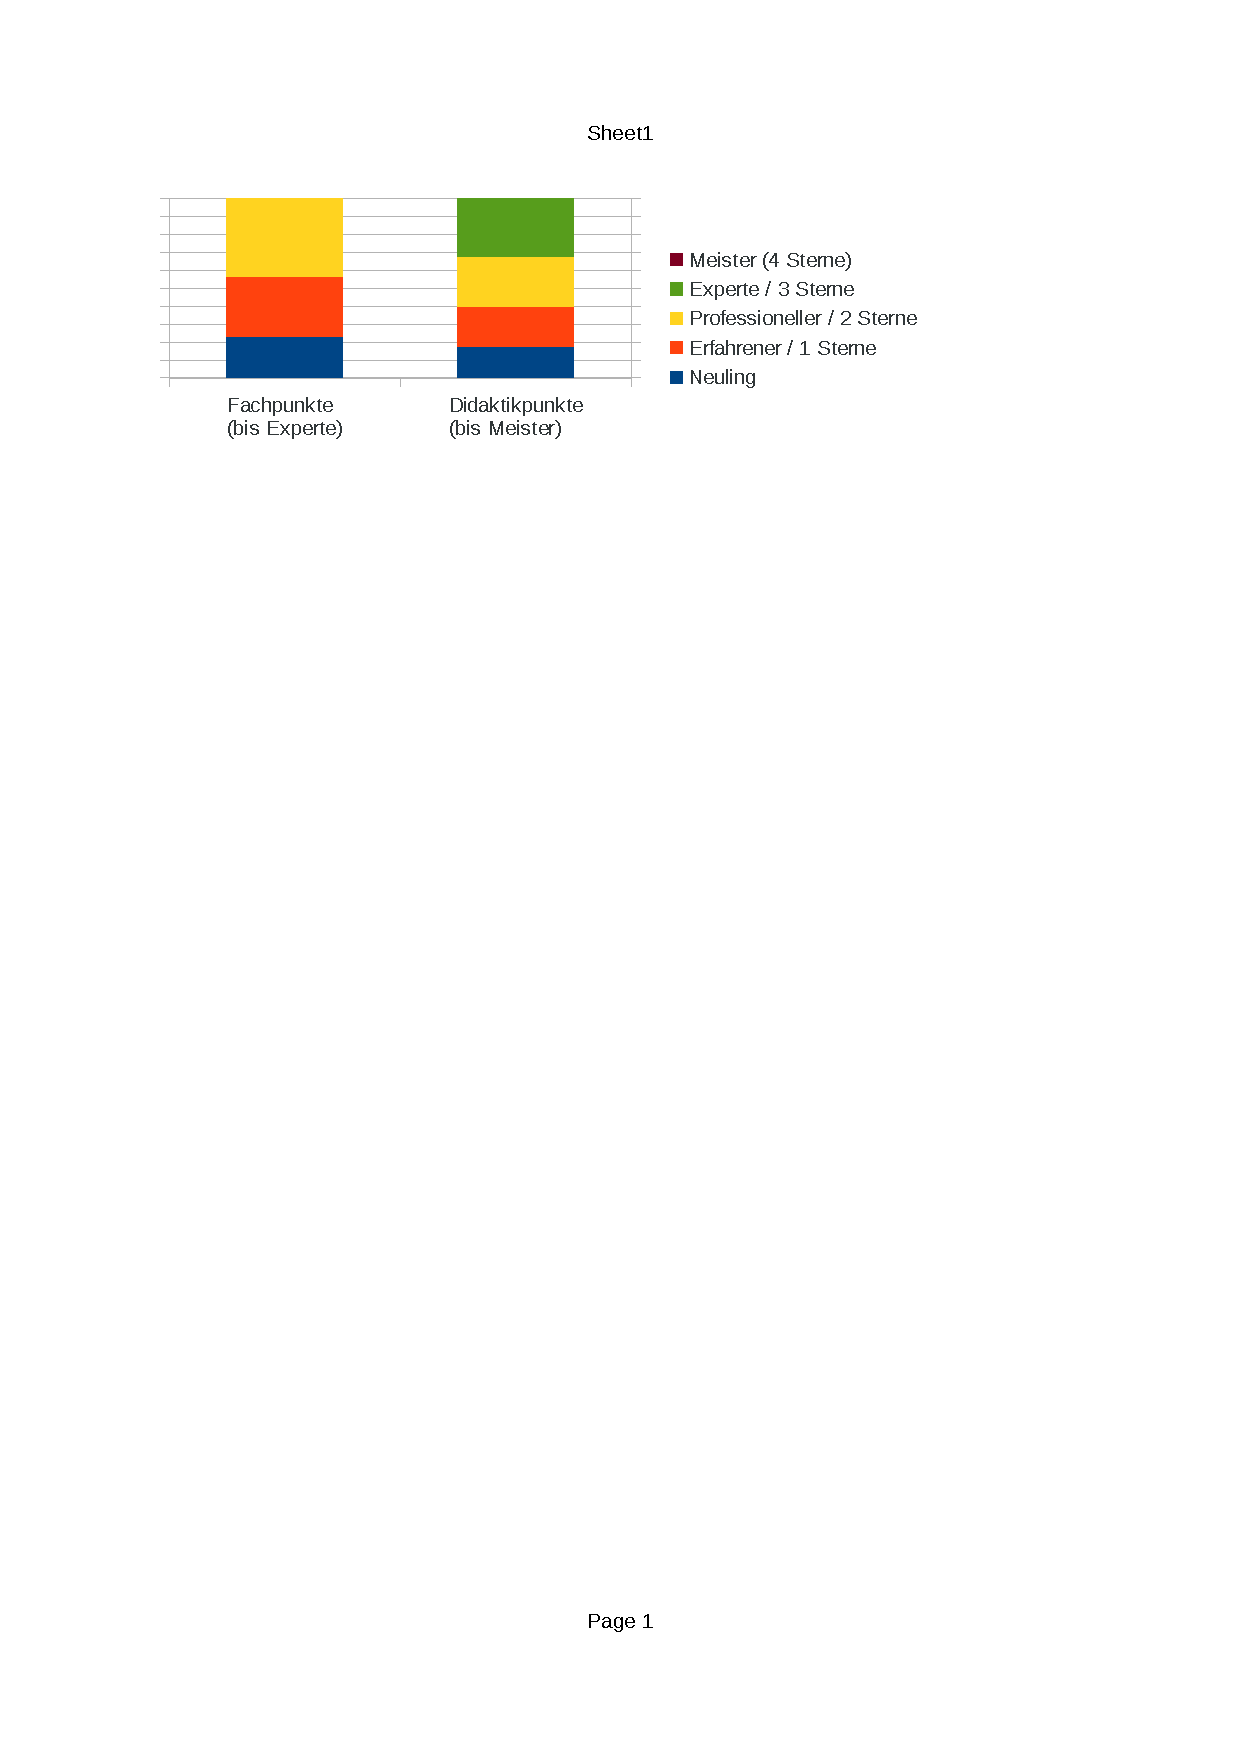
\includegraphics[width=1\textwidth]{verteilungDerPunkte.png}
\caption{Verteilung der Punkte}\label{ref:vertPunkt}
\end{figure}
Ein Meister hat durch das Erhalten der höchsten Wertung für die didaktische
Fähigkeit bereits bewiesen, dass er Spaß an der Vermittlung von Wissen hat.
Demnach bedarf er keiner weiteren Motivation eines höheren Ranges.
Vielmehr möchte er keine negativen Bewertungen seiner Lernenden erhalten und
bemüht sich der weiteren hochwertigen Qualität seiner Lerneinheiten.

\section{Rollen für Anwender}
Passend zum zuvor beschriebenen Konzept werden drei Rollen für Anwender
definiert. Dabei ist das Innehaben mehrerer Rollen zur gleichen Zeit ein Teil
des Modells. Zusammenfassend sind die Rechte und Pflichten eines Nutzers in den
verschieden Rollen in Tabelle \ref{tab:privilegesRoles} aufgeführt. Das dort
aufgeführte Forum ist nicht Teil der ersten produktiven Version (siehe
Abschnitt \ref{ref:weitereIdeen})

\subsection{Administrator}
Der Administrator ist der Verwalter der Plattform und damit für den
reibungslosen Ablauf seitens der Nutzer verantwortlich. Dazu kontrolliert er den
Zusammenhalt des Systems und greift bei inkonsistenzen oder Fehlern ein. Auch
bildet er die Schnittstelle zur Community, die sich in der Weiterentwicklung von
Masterly Mate engagiert.

\subsection{Lernender}
Der Lernende bildet die Hauptzielgruppe des Systems. Er soll WBTs finden, diese
durcharbeiten können und sich an Tutoren wenden, falls er auf ein Problem oder
Unklarheiten stößt. Dazu bietet Masterly Mate ihm das auffinden eines an sein
Fachwissen angepasstes Training. Weiterhin kann er Tutoren kontaktieren, die in
seinem Umkreis wohnen und passend zu seinem Rang Inhalte zu erläutern verstehen.
Die Lokation wird anhand der Postleitzahl festgemacht.

Ein Lernender kann in seinem fachlichen Level bis zum Experten aufsteigen.
Nähere Erläuterungen zu den fachlichen Rängen wurden in Abschnitt
\ref{ref:rankTopic} aufgeführt.

\subsection{Tutor}
Ein Lernender kann ab dem zweiten fachlichen Rang des Dreyfus-Modells (siehe
\ref{ref:dreyfus}) in seinem Profil die Einstellung "`Tutor"' anwählen. Damit
erscheint er unter den Suchergebnissen für Lernende, die einen Tutor suchen. Als
Tutor wird man von Lernenden gefunden, die Unterstützung in einem Fachgebiet
suchen.

\section{Dokumentation der API}
\begin {k}
mit "`rake doc:app"' lässt sich die Dokumentation erstellen

Verfügbar machen mit Link auf "`doc/app/index.html"'

Uebernimmt Julian?
\end{k}

\section{Automatisch generierte Filterung von Ergebnissen}
\begin{k}
\begin{itemize}
  \item Profilinfos werden ausgelesen und zur Eingrenzung der Ergebnisse
  verwendet
  \item daher kein Suchfeld nötig
\end{itemize}

Uebernimmt Benni
\end{k}

\section{Themen}
\begin{k}
Uebernimmt Benni
\end{k}